\documentclass[conference]{IEEEtran}
\IEEEoverridecommandlockouts
% The preceding line is only needed to identify funding in the first footnote. If that is unneeded, please comment it out.
\usepackage{cite}
\usepackage{amsmath,amssymb,amsfonts}
\usepackage{algorithmic}
\usepackage{graphicx}
\usepackage{textcomp}
\usepackage{xcolor}

\usepackage{multirow}
\usepackage{float}

\def\BibTeX{{\rm B\kern-.05em{\sc i\kern-.025em b}\kern-.08em
    T\kern-.1667em\lower.7ex\hbox{E}\kern-.125emX}}
\begin{document}

\title{Estimate Power generation of invisible solar site using State estimation\\
% {\footnotesize \textsuperscript{*}Note: Sub-titles are not captured in Xplore and
% should not be used}
\thanks{PEA, AIT, NEU}
}

\author{\IEEEauthorblockN{1\textsuperscript{st} Pornchai Chaweewat}
\IEEEauthorblockA{\textit{EECC} \\
\textit{AIT)}\\
Pathumthani, Thailand \\
chaweewat.p@gmail.com}
\and
\IEEEauthorblockN{2\textsuperscript{nd} Weerakorn Ongsakul}
\IEEEauthorblockA{\textit{EECC} \\
\textit{AIT)}\\
Pathumthani, Thailand \\
email address}
\and
\IEEEauthorblockN{3\textsuperscript{rd} Jai Govind Singh}
\IEEEauthorblockA{\textit{EECC} \\
\textit{AIT)}\\
Pathumthani, Thailand \\
email address}
\and
\IEEEauthorblockN{4\textsuperscript{th} Ali abur}
\IEEEauthorblockA{\textit{EEC} \\
\textit{NEU}\\
Boston, MA, USA \\
email address}
}

\maketitle

\begin{abstract}
The number of large scale and rooftop scale solar photovoltaic (PV) systems in electricity grid is growing at exponential rate.
Invisible solar PV refers to small-scale and rooftop solar sites in distribution system that are not mornitored by utilities.
These invisible solar PV sites cause challenging to utilies and system operators.
In this paper, a methodology is proposed to identify location and estimate installation capacity of solar PV sites.
With measurement voltage at any buses and power flow in any lines, state estimation (SE) algorithm could find power consumption in any buses.
The consumption are fed to find correlation with solar irradaiton data.
Thus, the correlative between these data could locate the site of invisible solar PV sites.
Futhermore, the change point method and proposed algorithm could estimate installation capacity of invisible solar PV sites.
The proposed methodology is test in distribution system i.e, four bus system and CIGRE Medium voltage distribution network with PV and Wind DER with randomly invsisble solar PV sites location.
The overall results of the study shows that the correlation between consumption and solar irradiation can perfectly identify invisible solar PV sites with $\text{F}_{1}$ score aboved 0.96 and Matthews correlation coefficient (MCC) score aboved 0.90.
The installation capacity estimation performe good with mean absolute error (MAPE) below 17\%.
\end{abstract}

\begin{IEEEkeywords}
  Solar photovoltaic, invisible solar PV site, Gaussian noise, state estimation, correlation, change point detection, Matthews correlation coefficient
\end{IEEEkeywords}


\section{Introduction}


Sixty years ago, the price of solar panels was astronomical.  The price was over 1,000 US dollars per watt in today's money with 1 percent efficiency~\cite{b18}.
As the cost continues to drop, solar panel systems are becoming much more viable for the average household.
Today's price is less than 2.8 US dollars per watt for solar panel system including solar module, inverter, wiring hardware, labor cost, and maintenance cost~\cite{b19}.
As result of exponentially acceralate increasing in number of globally solar PV integration, especailly in residential sector.


Many researchers have studied the impacts and risks of PV on distribution systems \cite{b20}-~\cite{b25}.
However, the detection and monitoring of residential PV systems has not been the focus of the studies and related research.

Recently, the highest penetration of solar PV, recognized a large number of unauthorized solar PV installation \cite{b26}.
Unauthorized solar PV installation creates safety risks and lack of visibility may result in incorrect planning, and operation, including over-voltage, back-feeding.
Futhermore, in worst case scenario, it may damange system equipment such as transformers, voltage regulators, as well as customer applicants \cite{b15}, \cite{b16}.
In previous studies, there are various reasons for unauthorized or incorrectly registered PV system:
a) owner decided not to apply for a permit to avoid fees \cite{b17},
b) regulations were required after the system was installed,
c) lack of awareness by the owner of diverse permitting rules,
d) difference rules depending on size and type of PV installation can make the owners believe they do not need a permit
e) change in property ownership including transfer,
f) multiple system installed or future iaddition at the same premise,
g) incorrect third party handling of the permit appication,
h) data entry and data maintenance errors.





The rest of the paper is structured as follows: Section II reviews related research on state estimation application for power system and previous detection and estimation techniques on invisible solar PV site.
Section III formulates the mathenatic model of measurement data as well as the structure of proposed method.
Section IV shows the results of proposed method on test cases.
Section V conclueds the paper and dicusses future research oppotunities on PV system detection and estimation.

\section{Literature reviews}

\subsection{Applications of State estimation in power system}



State estimation on distribution power system is reviewed in \cite{b9}.

State estimation provides the optimum estimate of power system state based on received measurement units and the knowledge of network modeling. The measurement units may include as follows:
\begin{itemize}
  \item power injection (real/reactive),
  \item power flow (real/reactive),
  \item bus voltage magnitude,
  \item phase angle,
  \item line current magnitude,
  \item current injection magnitude.
\end{itemize}

State Estimation provides various benefits for power system analysis as follows:

\subsubsection{Real time mornitoring}

For power system in transmission and distribution levels~\cite{b5}. The Advance Meter infrastructure (AMI) data are fed into SE to real-time mornitor distribution power system in\cite{b7}. It improved the accuracy comparing to pseudo measurment based on historical load.

\subsubsection{Load allocation}
In distribution power system, SE assigns active and reactive power values to bus downstream\cite{b6}. Class curves and individual average demand of clients improved accuracy of load allocation\cite{b4}.  The data from AMR system, which are used as the pseudo-measurements, was used to estimate load on the distribution transformers.\cite{b5}.

\subsubsection{Bad data analysis}

In several real application, it happens that some flow measurement has no sign or the sign is wrong.
A re-weighting technique was used to reduced the weights association to these measurements\cite{b6}.
It also could helps to treat of power flow with erroneous sign.
Futhurmore, SE was implemented in cyber attack events~\cite{b10} on power system states. A detection false data injection method is proposed in \cite{b8}.

\subsubsection{Topology indentification}

the status of branches and switches are indentified in\cite{b6}.


\subsection{previous solar PV detection techniques}
The previous studies has been done on detection of location and estimation of power generation of invisible solar PV sites.
Reference \cite{b11} proposed a change-point detection algorithm for a time series for residential solar PV detection. These method required smart meter data and historical load profile.
The uncertainty of solar PV site and the data generated by a small set of selected representative sites were taken into account to estimates the power gneneration of known solar PV site in~\cite{b12}.  The new hybrid k-means and PCA techniques provided good accuracy of estimating invisible solar PV sites.
The big data characterization of smart grids and two-layer dynamuc optimal synchrophasor measurement devices selection algorithm for fault detection, identification, and causal impact analysis was proposed in~\cite{b13}.
The utility data based on random matrix therory (RMT) are used in detection and estimation of invisible solar PV in real case in China in\cite{b14}.

\subsection{Contributions}
Many researchers have studied the detection and estimation location of invisible solar PV installation~\cite{b11}~\cite{b14}.
These study depended on smart meter data, data set of solar PV generation, as well as historical demand of customer in each load.
This paper proposed method which identify location using state estimation, correlation measured and estimating the installation capacity using change point method of invisible solar PV site.
All solar PV's site is assumed to operate at unity power factor.
The solar PV is located randomly at any bus excepted slack bus.
The measurement units are located at optimum locations.
The measured data such as solar irradiation, power flow measurements in lines and voltage measurements at busses are generated with gaussian noise.
The proposed method consists of four steps:
\begin{itemize}
  \item collect solar irradiation, measurement data
  \item allocate power demend in each buses, nodes.
  \item indentify invisible solar PV site
  \item estimate solar PV site's installation capacity
\end{itemize}

\section{Problem Formulation}

\begin{figure}[h!]
  \center
  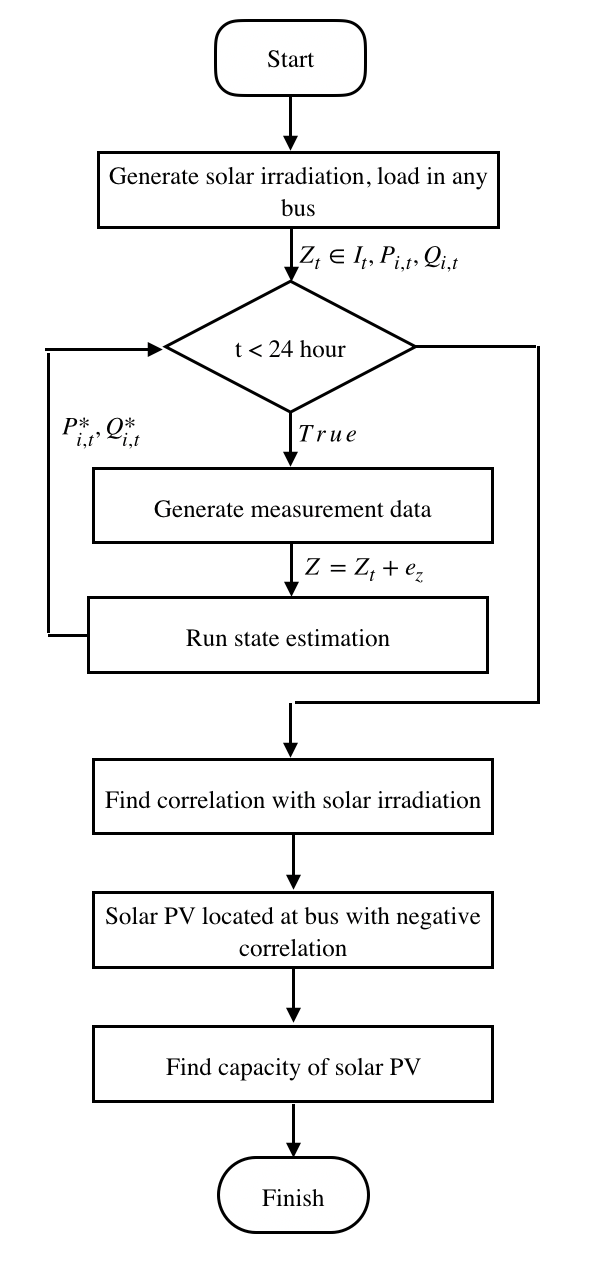
\includegraphics[scale=0.25]{images/conceptual_methodology.png}
  \caption{conceptual methodology}
  \label{fig.method}
\end{figure}

\subsection{Measurement devices, measured data and accuracy}

To generate measurement data for testing prurposes, measurement error was added to tha actual measurements as shown in Equation~\ref{eq.Z}.
\begin{equation}
  Z=Z_{a} \pm +e_{z}
\label{eq.Z}
\end{equation}
where $Z_{a}$ is actual data and $e_{z}$ is error added base on accuarcy of the measurement.
In this study, bus measurement has 3$\%$ error. line measurement has 5$\%$ error.

These error are assumed to be modeled independent Gaussian random variable\cite{b2}.
where where the error value is expected value from gaussian distribution.
noise is guassian distribution,as shown in Equation~\ref{eq.gaussian}
\begin{equation}
  g(x)=\frac{1}{\sigma \sqrt{2\pi}}e^{-\frac{1}{2}((x-\mu)/\sigma)^2}
  \label{eq.gaussian}
\end{equation}
\subsubsection{State variable description:} voltage, current, power flow from measurements devices

\subsection{Peform SE to find }
\subsubsection{LWS}
\subsubsection{Branch current, load allocation based state estimation}
is based on the weighted least square (WLS) approach\cite{b1}.
the method solves the following WLS problem to obtain an estimate ofthe system operating point defined by the system state x:
\begin{equation}
  \underset{x}{min} J(x)=\sum_{i=1}^{m}w_{i}(z_{i}-h_{i}(x))^{2}=\big[ z-h(x)\big]^{T}W\big[z-h(x)\big]
\label{eq.jacobian}
\end{equation}
where $w_{i}$ and $h_{i}(x)$ represent the weight and the measurements function associated with measurement $z_{i}$, respectively.
For the solution of this problem the conventional iterative method is adape by solving following normal equations at each iteration, to compute the update $x^{k+1}=x^{k}+\Delta x^{k}$
\begin{equation}
  \big[G(x^{k})\big]\Delta x^{k} = H^{T}(x^{k})W \big[ z-h(x^{k}) \big]
  \label(eq.delta_x)
\end{equation}

Where

\begin{equation}
  G(x)=H^{T}(x)WH(x)
  \label(eq.gain)
\end{equation}

is the gain matrix and H is the jacobian of the measurement function $h(x)$.

\subsection{Find correlation with solar irradiation}

A correlation is a statistical measure of relationship between two variables. The measure is best used in variables that demenstrate a linear relationship between each other.
The correlation coefficient that indicates the straength of the relationship between two variables can be found using following formula:

\begin{equation}
  \text{r}_{xy} =\frac{\sum(x_{i}-\overline{x})(y_{i}-\overline{y})}{\sqrt{\sum(x_{i}-\overline{y})^{2}(y_{i}-\overline{y})^{2})}}
  \label{eq.corr}
\end{equation}

where $\text{r}_{xy}$ is the correlation coefficient of the linear relationship between the variables x and y, $x_{i}$ is the values of the x-variable in a sample, $\overline{x}$ is the mean of the varialbes of the x-variable,
$y_{i}$ is the values of the y-variable in a sample, $\overline{y}$ is the mean of the varialbes of the y-variable.

The negaive correlation shows that the variables tend to move in opposity directions (i.e., when one variable increases, the other variable decreases).

\subsection{Find capacity of solar PV using changing point method}

\section{Test cases and Results}

  Two power system are tested. There two test cases are based on four bus system and CIGRE Task Force C6.04.02 paper\cite{b3}.

  \subsection{four bus system}
    The one line diagram of the four bus system is shown in Fig.~\ref{fig.4_bus_system}.

    \begin{figure}[H]
      \center
      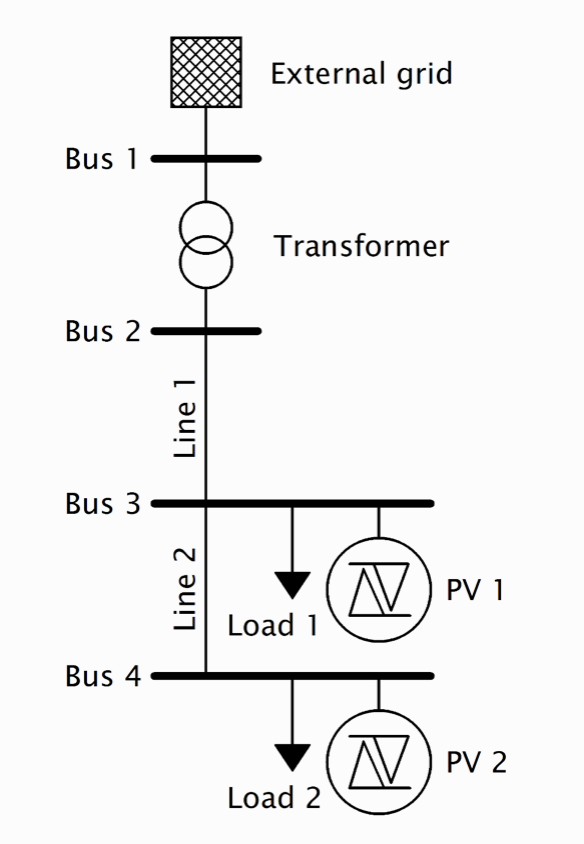
\includegraphics[scale=0.5]{images/four_bus_system.png}
      \caption{four bus system}
      \label{fig.4_bus_system}
    \end{figure}

    Table \ref{tab.Confusion_Matrix_4bus} shows the results. From the table, \ref{tab.Confusion_Matrix_4bus} it can be seen that the proposed method can predict perfectly location of invisible solar PV.
    \begin{table}[H]
      \centering
      \caption{Results of invisible solar PV identification on 4 bus system}
      \begin{tabular}{cc|c|c|}
        \cline{3-4}
                                                                                                                &     & \multicolumn{2}{l|}{Actual PV located} \\ \cline{3-4}
                                                                                                                &     & Yes                & No                \\ \hline
        \multicolumn{1}{|l|}{\multirow{2}{*}{\begin{tabular}[c]{@{}l@{}}Prediction \\ PV located\end{tabular}}} & Yes & 126                & 0                \\ \cline{2-4}
        \multicolumn{1}{|l|}{}                                                                                  & No  & 9                  & 60                \\ \hline
      \end{tabular}
      \label{tab.Confusion_Matrix_4bus}
    \end{table}
    The results is tested by $\text{F}_{1}$ score and MCC using Equation~\ref{eq.F_1_score}, \ref{eq.MCC}.
    The $\text{F}_{1}$ score is 0.965. The MCC is 0.901
    The false negative (FN) occurs when invisible solar PV's capacity is 1-2 kW where maximum demand is around 30 kW.

    \begin{table}[H]
      \centering
      \caption{Results of invisible solar PV estimation on 4 bus system}
      \begin{tabular}{ccc}
        \hline
        Size of invisible solar PV (kW) & MAE(kW) & MAPE (\%) \\
        \hline
        1-10                  & 0.77            & 13.9            \\
        11-20                 & 2.4             & 16.9            \\
        21-30                 & 3.75            & 14.2            \\
        31-40                 & 4.42            & 12              \\
        41-50                 & 3.85            & 8.4\\
        \hline
      \end{tabular}
      \label{tab.Error_4bus}
    \end{table}
    The overall MAPE is 13.587 \% and MAE is 2.919 kW.



  \subsection{CIGRE system}

    \begin{figure}[H]
      \center
      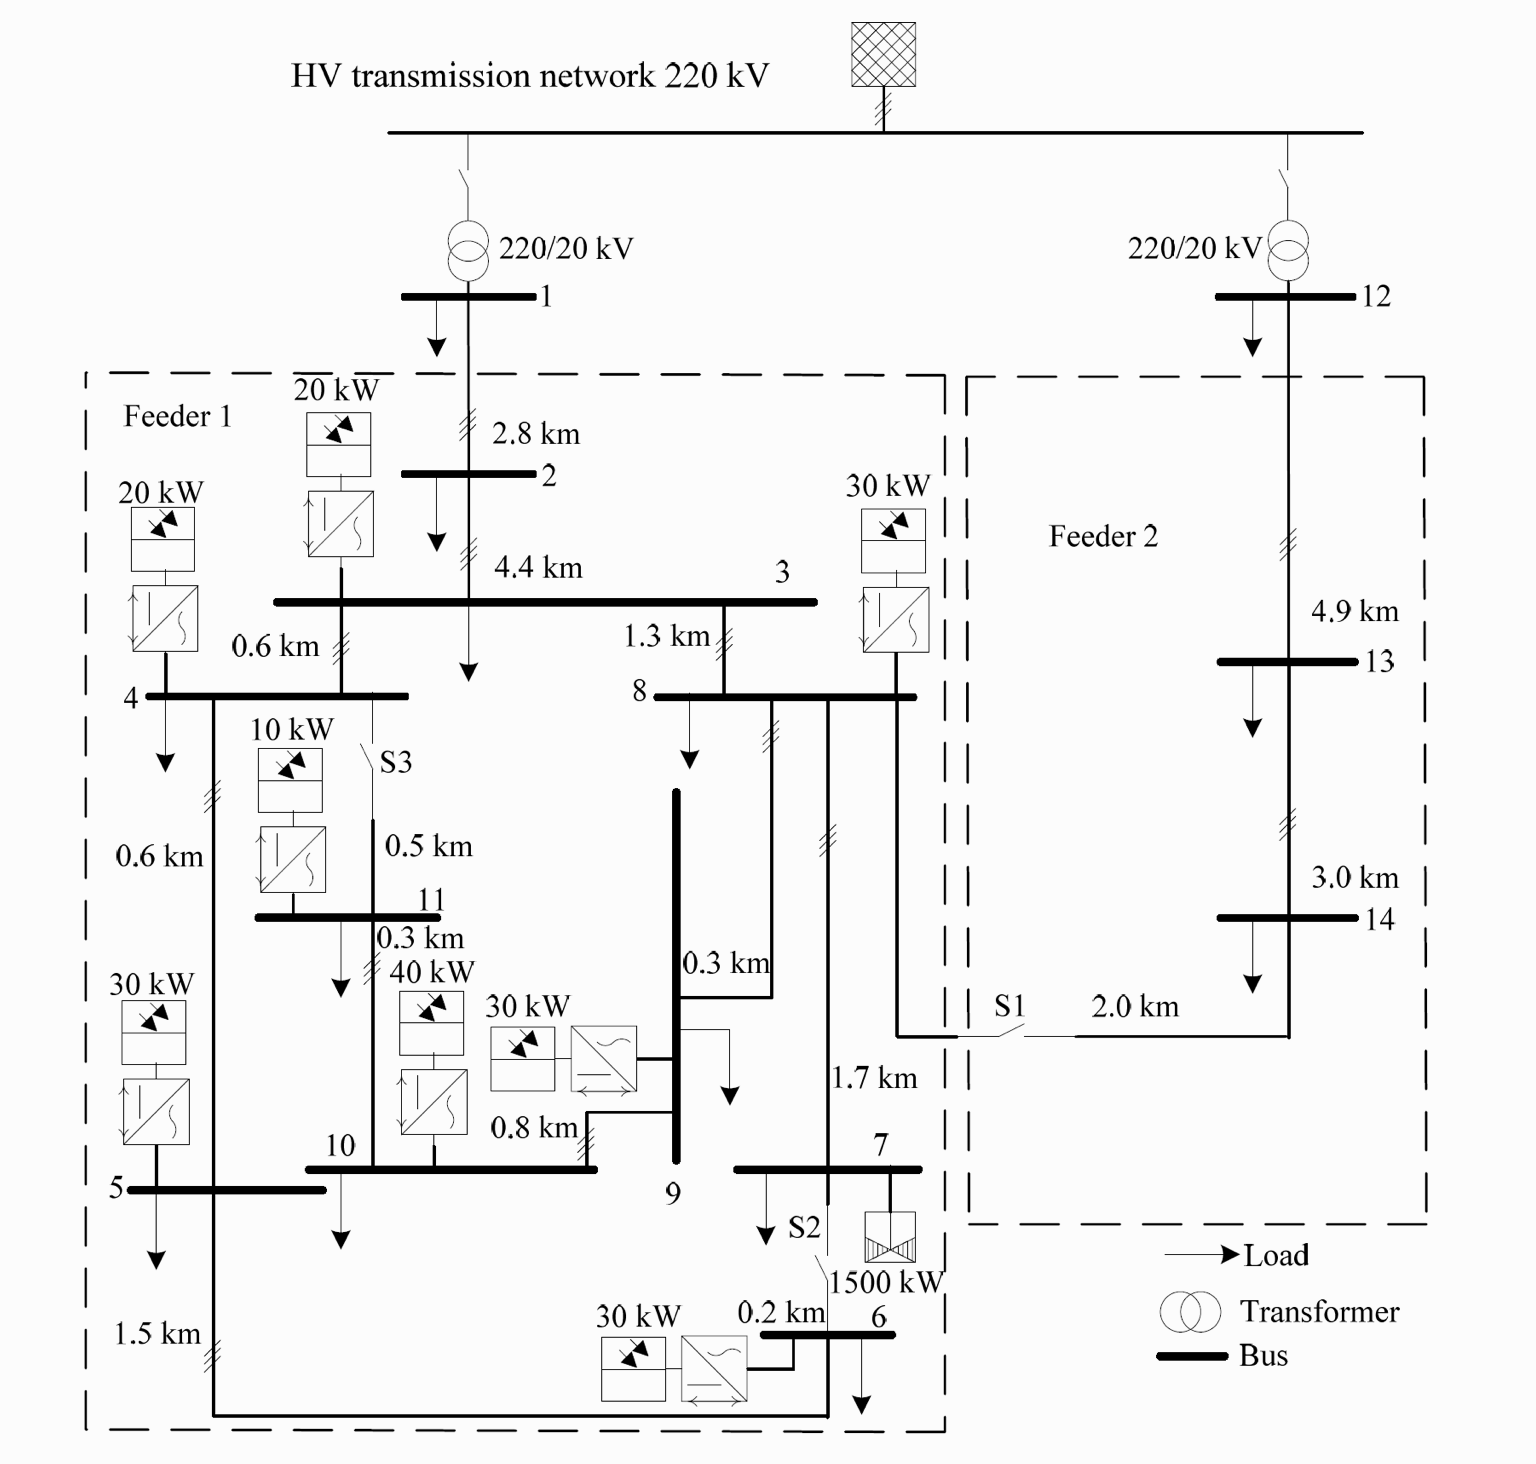
\includegraphics[scale=0.25]{images/CIGRE_network.png}
      \caption{CIGRE network}
      \label{fig.CIGRE_network}
    \end{figure}

    Table \ref{tab.Confusion_Matrix_CIGRE} shows the results. From the table, \ref{tab.Confusion_Matrix_4bus} it can be seen that the proposed method can predict perfectly location of invisible solar PV.

    \begin{table}[H]
      \centering
      \caption{Results of invisible solar PV identification on CIGREsystem}
      \begin{tabular}{cc|c|c|}
        \cline{3-4}
                                                                                                                &     & \multicolumn{2}{l|}{Actual PV located} \\ \cline{3-4}
                                                                                                                &     & Yes                & No                \\ \hline
        \multicolumn{1}{|l|}{\multirow{2}{*}{\begin{tabular}[c]{@{}l@{}}Prediction \\ PV located\end{tabular}}} & Yes & 154                & 8                 \\ \cline{2-4}
        \multicolumn{1}{|l|}{}                                                                                  & No  & 3                  & 159                \\ \hline
      \end{tabular}
      \label{tab.Confusion_Matrix_CIGRE}
    \end{table}

    The results is tested by $\text{F}_{1}$ score and MCC using Equation~\ref{eq.F_1_score}, \ref{eq.MCC}.
    The $\text{F}_{1}$ score is 0.965. The MCC is 0.9325.
    The false negative (FN) occurs when invisible solar PV's capacity is 10-20 kW.

    \begin{table}[H]
      \centering
      \caption{Results of invisible solar PV estimation on CIGRE system}
      \begin{tabular}{ccc}
        \hline
        Size of invisible solar PV (kW) & MAE (kW) & MAPE (\%) \\
        \hline

        1-100                  & 9.01            & 17.60            \\
        101-200                 & 24.3            & 15.97            \\
        201-300                & 50.00            & 19.85            \\
        301-400               & 52.55            & 13.98             \\
        401-500              & 54.92            & 12.28 \\
        \hline

      \end{tabular}
      \label{tab.Error_CIGRE}
    \end{table}

    The overall MAPE is 16.27 \% and MAE is 37.58 kW.

\section{Conclusion}
Here is Conclusion.
\section*{Acknowledgment}

\begin{thebibliography}{00}
  \bibitem{b18} https://www.theguardian.com/sustainable-business/2016/jan/31/solar-power-what-is-holding-back-growth-clean-energy
  \bibitem{b19} https://blog.pickmysolar.com/the-price-of-a-solar-panel-system-over-the-years
  \bibitem{b20} M. E. Baran, H. Hooshyar, Z. Shen, and A. Huang, “Accommodating high PV penetration on distribution feeders,” IEEE Trans. Smart Grid, vol. 3, no. 2, pp. 1039–1046, Jun. 2012.
  \bibitem{b21}  M. J. Reno, K. Coogan, R. J. Broderick, J. Seuss, and S. Grijalva, “Impact of PV variability and ramping events on distribution voltage regulation equipment,” in Proc. IEEE Photovolt. Spec. Conf., Tampa, FL, USA, 2014.
  \bibitem{b22} M. E. Baran, H. Hooshyar, Z. Shen, and A. Huang, “Accommodating high PV penetration on distribution feeders,” IEEE Trans. Smart Grid, vol. 3, no. 2, pp. 1039–1046, Jun. 2012.
  \bibitem{b23} P. Li, X. Yu, J. Zhang, and Z. Yin, “The H∞ control method of grid- tied photovoltaic generation,” IEEE Trans. Smart Grid, vol. 6, no. 4, pp. 1670–1677, Jul. 2015.
  \bibitem{b24}  A. Samadi, L. Söder, E. Shayesteh, and R. Eriksson, “Static equivalent of distribution grids with high penetration of PV systems,” IEEE Trans. Smart Grid, vol. 6, no. 4, pp. 1763–1774, Jul. 2015.
  \bibitem{b25}  H. Ravindra et al.,“Impact of PV on distribution protection system,” in Proc. North Amer. Power Symp. (NAPS), Champaign, IL, USA, Sep. 2012, pp. 1–6.
  \bibitem{b26} P. Fairley. (Jan. 2015). Hawaii’ s Solar Push Strains the Grid. [online]. Available: http://www.technologyreview.com/news/534266/ hawaiis-solar-push-strains-the-grid/
  \bibitem{b15} W. Staff. (Sep. 2014). Heco Customers Asked to Disconnect Unauthorized PV Systems. [Online]. Available: http://khon2.com/2014/ 09/05/heco-customers-asked-to-disconnect-unauthorized-pv-systems/
  \bibitem{b16} V. Schwarzer and R. Ghorbani, “Transient over-voltage mitiga- tion: Explanation and mitigation options for inverter-based dis- tributed generation projects,” Elect.Vehicle Transp. Center, Sch. Ocean Earth Sci. Technol., Univ. Hawai’ i Manoa, Honolulu, HI, US A , Tech. Rep. HNEI-02-15, Feb. 2014.
  \bibitem{b17} https://www.snopes.com/fact-check/is-it-illegal-florida-power-home-solar-storm/
  \bibitem{b1} Roytelman I. and S.M. Shahidehpour, ‘State estimation for electric power distribution systems in quasi real-time conditions’, IEEE Trans. Power Systems, 1993 winter meeting, paper no:090-1-PW RD.
  \bibitem{b2} A. Abur and A. G. Exposito, Power System State Estimation: Theory and Implementation. New York: Marcel Dekker, 2004.
  \bibitem{b3} CIGRE' Task Force C6.04.02: Developing benchmark models for integrating distributed energy resourcesS. Barsali, Kai Strunz, Zbigniew StyczynskiPublished 2005
  \bibitem{b4} STATE ESTIMATION FOR LOAD ALLOCATION IN DISTRIBUTION POWER SYSTEMS, R. Sharifian 1 E. Jafari 1 M. Rahimi 2 P. Ghaebi Panah 3
  \bibitem{b5} A Revised Branch Current-Based Distribution System State Estimation Algorithm and Meter Placement Impact, Haibin Wang, Student Member, IEEE, and Noel N. Schulz, Senior Member, IEEE
  \bibitem{b6} An Integrated Load AllocatiodState Estimation Approach for Distribution Networks, JorgePereira, J. T. Saraiva,Member, IEEE, V. Miranda, Member, IEEE
  \bibitem{b7} Distribution System State Estimation Using AMI Data, Mesut Baran, T. E. McDermott
  \bibitem{b8} Gu Chaojun, Student Member, IEEE, Panida Jirutitijaroen, Senior Member, IEEE, and Mehul Motani, Member, IEEE, Detecting False Data Injection Attacks in AC State Estimation
  \bibitem{b9} A Review on Distribution System State Estimation, Anggoro Primadianto and Chan-Nan Lu, Fellow, IEEE
  \bibitem{b10} Nathan Wallace, Stanislav Ponomarev, and Travis Atkison, Identification of Compromised Power System State Variables
  \bibitem{b11} X. Zhang and S. Grijalva, “A data-driven approach for detection and estimation of residential pv installations,” IEEE Transactions on Smart Grid, vol. 7, no. 5, pp. 2477–2485, Sept 2016.
  \bibitem{b12} H. Shaker, H. Zareipour, and D. Wood, “Estimating power generation of invisible solar sites using publicly available data,” IEEE Transactions on Smart Grid, vol. 7, no. 5, pp. 2456–2465, Sept 2016.
  \bibitem{b13} H. Jiang, X. Dai, D. W. Gao, J. J. Zhang, Y. Zhang, and E. Muljadi, “Spatial-temporal synchrophasor data characterization and analytics in smart grid fault detec- tion, identification, and impact causal analysis,” IEEE Transactions on Smart Grid, vol. 7, no. 5, pp. 2525– 2536, Sept 2016.
  \bibitem{b14} Detection and Estimation of the Invisible Units Using Utility Data Based on Random Matrix Theory, Xing He, Robert C. Qiu, Fellow, IEEE, Lei Chu, Qian Ai, Zenan Ling, Jian Zhang
\end{thebibliography}






\end{document}
